\chapter{Dados}

Neste trabalho foram utilizados dois conjuntos de dados compostos da sequência de aminoácidos de proteínas com estruturas resolvidas experimentalmente e da estrutura secundária atribuída aos seus resíduos por quatro diferentes algoritmos: DSSP \cite{Kabsch:1978}, Stride \cite{Frishman:1990}, Kaksi \cite{Martin:2000} e PROSS\cite{Srinivasan:1994}.

O primeiro conjunto selecionado é formado por um grande número de estruturas de alta qualidade e tem como finalidade ser utilizado na busca de regras gerais para o autômato celular. Essas regras gerais são um dos elementos mais importantes desse trabalho, pois permitem avaliar a generalização do autômato celular, isto é, qual o grau de sucesso da aplicação do autômato celular para o universo de proteínas existentes.

O segundo conjunto selecionado é composto de quatro proteínas com altíssima identidade sequêncial e diferentes estruturas terciárias e secundárias. Esse conjunto foi selecionado por ser, possivelmente, o caso experimental mais desafiador para os métodos de predição de estrutura secundária. Como discutiremos ao longo do texto, todos os métodos de predição de estrutura secundária, assim como os de modelagem comparativa, tendem a falhar nesse conjunto devido à limitações teóricas dos métodos.

\section{Proteínas com altíssima identidade sequêncial e diferentes estruturas terciárias e secundárias}

Em 2007, Alexander e colaboradores \cite{17609385}, desenharam um experimento onde obtiveram dois enovelamentos com topologias diferentes para sequências com mais de 88\% de identidade sequencial. O ponto de partida do experimento foram dois domínios chamados $G_A$ e $G_B$  com 56 aminoácidos.  O domínio $G_A$ possui um feixe de 3 hélices $\alpha$ (\textit{3-$\alpha$ helix bundle}) enquanto o domínio $G_B$ apresenta a enovelamento 4$\beta$+$\alpha$, ou seja, 4 fitas $\beta$ mais uma hélice $\alpha$ (Figura \ref{fig:ga_gb}).

\begin{figure}
  \centering
  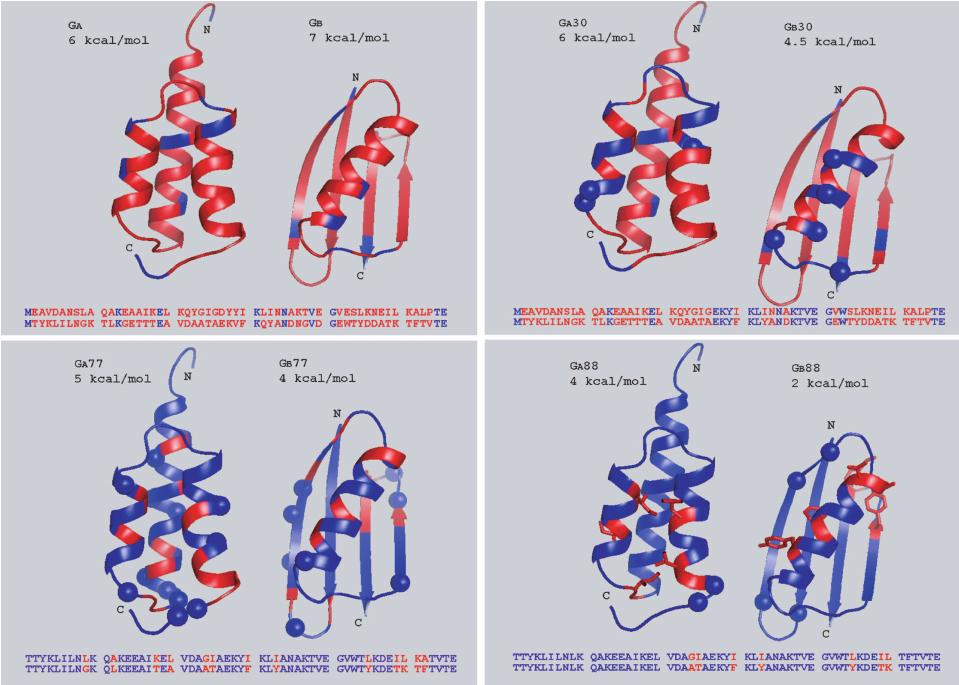
\includegraphics[width=1.0\textwidth]{figures/ga_gb.jpg}
  \caption{Figura da sequencia e das estruturas das camaleonicas}
        \label{fig:ga_gb}
\end{figure}

Posteriormente, uma série de outros estudos sobre esses dois domínios demonstrou ser possível obter os dois enovelamentos com idetidade sequencial ainda maiores \cite{10.1073/pnas.0805857105, 10.1073/pnas.0906408106}.  Até que em 2012, He e colaboradores \cite{10.1016/j.str.2011.11.018}, obtiveram mutações pontuais capazes de alterar a estrutura entre os dois enovelamentos (Figura \ref{fig:camaleonicas}). As estruturas resolvidas por RMN das quatro proteínas foram as utilizadas para compor esse conjunto de dados ( PDB IDs: 2LHC, 2LHD, 2LHE, 2LHG) utilizando os 10 primeiros modelos de cada estruturas com o objetivo de manter um equilíbrio nos dados.

\begin{figure}
	\centering
	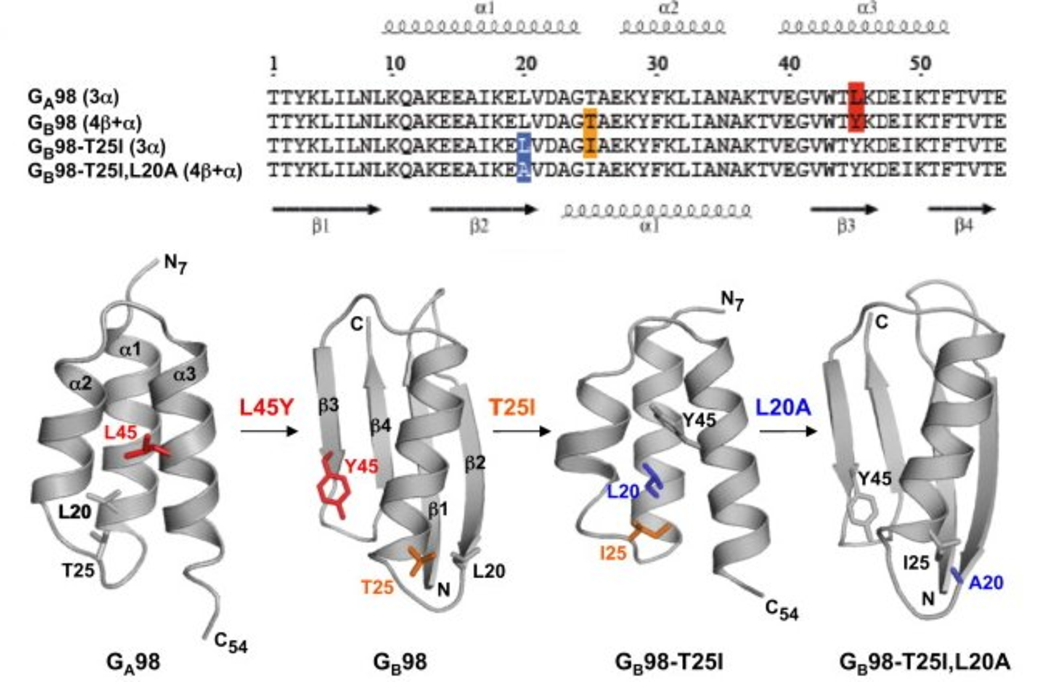
\includegraphics[width=1.0\textwidth]{figures/chameleonic_resume.pdf}
	\caption{Figura da sequencia e das estruturas das camaleonicas}
        \label{fig:camaleonicas}
\end{figure}

\section{Proteínas  diversas}

O conjunto de proteínas diversas utilizado para o treinamento do autômato celular foi obtido do banco de dados “Top8000” (versão de 2015). Esse banco de dados foi organizado pelo Richardson Lab da Universidade de Duke (disponível em \href{https://github.com/rlabduke/reference_data}{github.com/rlabduke/reference\_data}). As cadeias selecionadas atendem aos seguintes critérios:

\begin{itemize}
	\item{Resolução < 2.0 \AA}
	\item{MolProbity score < 2.0}
	\item{$\le 5 \%$ dos resíduos apresentando comprimentos de ligação anormais ( $> 4\sigma$)}
	\item{$\le 5 \%$ dos resíduos apresentando ângulos de ligação anormais ( $> 4\sigma$)}
	\item{$\le 5 \%$ dos resíduos com desvios anormais do  $C_\beta$ ( > 0.25 \AA)}
\end{itemize}

As cadeias selecionadas pelos critérios acima são subagrupadas de acordo com o grau de identidade sequencial (homologia): < 50\%, <70\% e <95\%.  Cadeias que apresentavam resíduos indeterminados na estrutura ou que apresentaram algum erro durante a atribuição da estrutura secundária por algum dos quatro métodos foram removidos do conjunto. A tabela \ref{tab:example} mostra o número de cadeias utilizadas.

\begin{table}
    \myfloatalign
  \begin{tabularx}{\textwidth}{Xll} \toprule
    \tableheadline{Conjunto}   & \tableheadline{\# original}   & \tableheadline{\# utilizadas}  \\ 
    \midrule
    Top8000-hom50 & 7233 &  6749 \\
    Top8000-hom70 & 7958 & 7435 \\
    Top8000-hom95 & 8826 & 8227 \\
    %autem vulputate ex & parola & romanic \\
    %usu mucius iisque & studio & sanctificatef \\
    \bottomrule
  \end{tabularx}
  \caption[Autem timeam deleniti usu id]{Número de cadeias presentes no banco de dados Top8000 (Richardson Lab) e número de cadeias utilizadas neste trabalho após a exclusão de cadeias que apresentaram algum problema durante a atribuição da estrutura secundária ou que possuiam resíduos indeterminados.}  \label{tab:example}
\end{table}

